\chapter{Funksjonsegenskaper}
\begin{table}[H]
  \centering
  \caption{Function Properties and Optimization Methods}
  \footnotesize
  \begin{tabularx}{\textwidth}{@{} >{\RaggedRight}Z Y Y Y Y Y Y Y @{}}
    \toprule
    \textbf{Function (Domain)}                                                        & \textbf{Cvx} & \textbf{Coe} & \textbf{lsc} & \textbf{QCvx} & \textbf{Loc} & \textbf{Glo} & \textbf{Alg}         \\
    \midrule
    \multicolumn{8}{@{}l}{\textbf{Scalar Functions (\(\R\))}}                                                                                                                                           \\
    \midrule
    \( f(x) = x^2 \)                                                                  & \yes         & \yes         & \yes         & \yes          & \yes         & \yes         & Gradient Descent     \\
    \( f(x) = |x| \)                                                                  & \yes         & \yes         & \yes         & \yes          & \yes         & \yes         & Proximal/Subgradient \\
    \( f(x) = x^3 \)                                                                  & \no          & \no          & \yes         & \no           & \no          & \no          & Heuristics           \\
    \( f(x) = x^4 - Cx^2 \)                                                           & \no          & \yes         & \yes         & \no           & \yes         & \yes         & Newton               \\
    \( f(x) = \begin{cases} 0 & x \leq 0 \\ 1 & x > 0 \end{cases} \)                  & \no          & \no          & \yes         & \yes          & \yes         & \yes         & Subgradient          \\

    \( f(x) = \sqrt{x}\ (x \geq 0) \)                                                 & \no          & \no          & \yes         & \yes          & \yes         & \yes         & Gradient Descent     \\
    \( f(x) = \log(1 + e^x) \)                                                        & \yes         & \yes         & \yes         & \yes          & \yes         & \yes         & Gradient Descent     \\
    \( f(x) = Ce^x \)                                                                 & \yes         & \no          & \yes         & \yes          & \no          & \no          & Heuristics           \\
    \( f(x) = e^x - x \)                                                              & \yes         & \yes         & \yes         & \yes          & \yes         & \yes         & Newton               \\
    \( f(x) = \sin(x) \)                                                              & \no          & \no          & \yes         & \no           & \yes         & \yes         & Heuristics           \\

    \midrule

    \multicolumn{8}{@{}l}{\textbf{Vector Functions (\(\R^d\))}}                                                                                                                                         \\
    \midrule
    \( f(\mathbf{x}) = \|\mathbf{x}\| \)                                              & \yes         & \yes         & \yes         & \yes          & \yes         & \yes         & Proximal             \\
    \( f(\mathbf{x}) = \|\mathbf{x}\| + \sin(x_1) \)                                  & \no          & \yes         & \yes         & \no           & \yes         & \yes         & Stochastic GD        \\
    \( f(\mathbf{x}) = \mathbf{x}^\top \mathbf{A} \mathbf{x}\ (\mathbf{A} \succ 0) \) & \yes         & \yes         & \yes         & \yes          & \yes         & \yes         & Newton               \\
    \midrule

    \multicolumn{8}{@{}l}{\textbf{Counterexamples}}                                                                                                                                                     \\
    \midrule
    \( f(x) = \sqrt{|x|} \)                                                           & \no          & \no          & \yes         & \yes          & \yes         & \yes          & Heuristics           \\
    \( f(x,y) = x^4y^2 + x^4 - 2x^3y \)                                               & \no          & \yes         & \yes         & \no           & \yes         & \yes         & Evolutionary         \\
    \bottomrule
  \end{tabularx}
  \label{tab:function_properties}
\end{table}


\newpage


\begin{table}[ht]
  \centering
  \scriptsize
  \begin{tabular}{|c|c|c|c|c|}
    \hline
    \rowcolor{gray!20}
    \textbf{\color{thm-color!20}Name} & \textbf{\color{thm-color!20}Equation \( f(x,y) \)} & \textbf{\color{thm-color!20}Description} & \textbf{\color{thm-color!20}Key Features} & \textbf{\color{thm-color!20}Plot} \\
  \hline
  \textbf{Plane} & \( z = 2x + 3y + 1 \) & Flat surface & Linear in \(x\) and \(y\) & 
  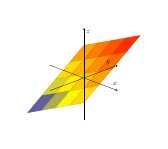
\begin{tikzpicture}[scale=0.25]
  \begin{axis}[
    view={45}{30},
    xlabel=$x$,
    ylabel=$y$,
    zlabel=$z$,
    axis lines=middle,
    ticks=none,
    enlargelimits=true,
    axis on top,
    z post scale=1.5,
]
  \addplot3[surf, domain=-2:2, samples=5] {2*x + 3*y + 1};
  \end{axis}
  \end{tikzpicture} \\
  \hline
  
  \textbf{Elliptic Paraboloid} & \( z = x^2 + y^2 \) & Bowl opening upward & Circular contours & 
  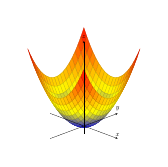
\begin{tikzpicture}[scale=0.25]
  \begin{axis}[
    view={45}{30},
    xlabel=$x$,
    ylabel=$y$,
    zlabel=$z$,
    axis lines=middle,
    ticks=none,
    enlargelimits=true,
    axis on top,
    z post scale=1.5,
    xlabel style={anchor=south},
    ylabel style={anchor=south},
    zlabel style={anchor=south},
    clip=false
]
  \addplot3[surf, domain=-2:2, samples=20] {x^2 + y^2};
  \end{axis}
  \end{tikzpicture} \\
  \hline
  
  \textbf{Hyperbolic Paraboloid} & \( z = x^2 - y^2 \) & Saddle shape & Hyperbolic cross-sections & 
  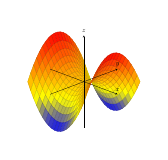
\begin{tikzpicture}[scale=0.25]
  \begin{axis}[
    view={45}{30},
    xlabel=$x$,
    ylabel=$y$,
    zlabel=$z$,
    axis lines=middle,
    ticks=none,
    enlargelimits=true,
    axis on top,
    z post scale=1.5,
    xlabel style={anchor=south},
    ylabel style={anchor=south},
    zlabel style={anchor=south},
    clip=false
]
  \addplot3[surf, domain=-2:2, samples=20] {x^2 - y^2};
  \end{axis}
  \end{tikzpicture} \\
  \hline
  
  \textbf{Rotated Saddle} & \( z = xy \) & Diagonal saddle & Cross-term \(xy\) dominates & 
  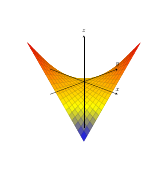
\begin{tikzpicture}[scale=0.25]
  \begin{axis}[
    view={45}{30},
    xlabel=$x$,
    ylabel=$y$,
    zlabel=$z$,
    axis lines=middle,
    ticks=none,
    enlargelimits=true,
    axis on top,
    z post scale=1.5,
    xlabel style={anchor=south},
    ylabel style={anchor=south},
    zlabel style={anchor=south},
    clip=false
]
  \addplot3[surf, domain=-2:2, samples=20] {x*y};
  \end{axis}
  \end{tikzpicture} \\
  \hline
  
  \textbf{Cone} & \( z = \sqrt{x^2 + y^2} \) & Double-napped cone & Linear scaling & 
  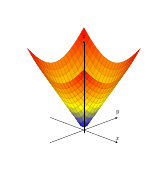
\begin{tikzpicture}[scale=0.25]
  \begin{axis}[
    view={45}{30},
    xlabel=$x$,
    ylabel=$y$,
    zlabel=$z$,
    axis lines=middle,
    ticks=none,
    enlargelimits=true,
    axis on top,
    z post scale=1.5,
    xlabel style={anchor=south},
    ylabel style={anchor=south},
    zlabel style={anchor=south},
    clip=false
]
  \addplot3[surf, domain=-2:2, samples=20] {sqrt(x^2 + y^2)};
  \end{axis}
  \end{tikzpicture} \\
  \hline
  
  \textbf{Ellipsoid} & \( z = \sqrt{1 - x^2 - y^2} \) & Hemisphere & Circular domain & 
  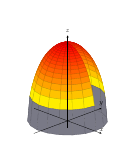
\begin{tikzpicture}[scale=0.25]
  \begin{axis}[
    view={45}{30},
    xlabel=$x$,
    ylabel=$y$,
    zlabel=$z$,
    axis lines=middle,
    ticks=none,
    enlargelimits=true,
    axis on top,
    z post scale=1.5,
    xlabel style={anchor=south},
    ylabel style={anchor=south},
    zlabel style={anchor=south},
    clip=false
]
  \addplot3[surf, domain=0:1, samples=20, y domain=0:360] ({x*cos(y)}, {x*sin(y)}, {sqrt(1 - x^2)});
  \end{axis}
  \end{tikzpicture} \\
  \hline
  
  \textbf{Hyperboloid (1-Sheet)} & Parametric: 
  \(\begin{aligned} 
  x &= \cosh u \cos v \\[-0.2em]
  y &= \cosh u \sin v \\[-0.2em]
  z &= \sinh u 
  \end{aligned}\) & Hourglass shape & One surface & 
  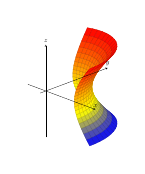
\begin{tikzpicture}[scale=0.25]
  \begin{axis}[
    view={45}{30},
    xlabel=$x$,
    ylabel=$y$,
    zlabel=$z$,
    axis lines=middle,
    ticks=none,
    enlargelimits=true,
    axis on top,
    z post scale=1.5,
    xlabel style={anchor=south},
    ylabel style={anchor=south},
    zlabel style={anchor=south},
    clip=false
]
  \addplot3[surf, domain=-1:1, y domain=0:360, samples=20] 
  ({cosh(x)*cos(deg(y))}, {cosh(x)*sin(deg(y))}, {sinh(x)});
  \end{axis}
  \end{tikzpicture} \\
  \hline
  
  \textbf{Hyperboloid (2-Sheets)} & \( z = \sqrt{x^2 - y^2 - 1} \) & Two surfaces & \(x^2 - y^2 \geq 1\) & 
  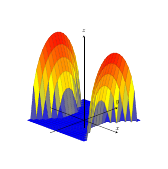
\begin{tikzpicture}[scale=0.25]
  \begin{axis}[
    view={45}{30},
    xlabel=$x$,
    ylabel=$y$,
    zlabel=$z$,
    axis lines=middle,
    ticks=none,
    enlargelimits=true,
    axis on top,
    z post scale=1.5,
    xlabel style={anchor=south},
    ylabel style={anchor=south},
    zlabel style={anchor=south},
    clip=false
]
  \addplot3[surf, domain=-2:2, samples=20,
            restrict expr to domain={sqrt(x^2-y^2-1)}{0:10}] {sqrt(max(x^2-y^2-1,0))};
  \end{axis}
  \end{tikzpicture} \\
  \hline
  
  \textbf{Circular Cylinder} & Parametric: 
  \(\begin{aligned} 
  x &= \cos\theta \\[-0.2em]
  y &= \sin\theta \\[-0.2em]
  z &= z 
  \end{aligned}\) & Infinite tube & Extruded circle & 
  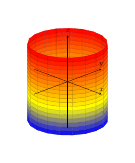
\begin{tikzpicture}[scale=0.25]
  \begin{axis}[
    view={45}{30},
    xlabel=$x$,
    ylabel=$y$,
    zlabel=$z$,
    axis lines=middle,
    ticks=none,
    enlargelimits=true,
    axis on top,
    z post scale=1.5,
    xlabel style={anchor=south},
    ylabel style={anchor=south},
    zlabel style={anchor=south},
    clip=false
]
  \addplot3[surf, domain=0:360, y domain=-2:2, samples=20] ({cos(x)}, {sin(x)}, {y});
  \end{axis}
  \end{tikzpicture} \\
  \hline
  
  \textbf{Parabolic Cylinder} & \( z = x^2 \) & U-shaped trough & Extruded parabola & 
  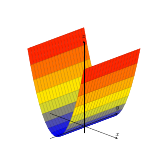
\begin{tikzpicture}[scale=0.25]
  \begin{axis}[
    view={45}{30},
    xlabel=$x$,
    ylabel=$y$,
    zlabel=$z$,
    axis lines=middle,
    ticks=none,
    enlargelimits=true,
    axis on top,
    z post scale=1.5,
    xlabel style={anchor=south},
    ylabel style={anchor=south},
    zlabel style={anchor=south},
    clip=false
]
  \addplot3[surf, domain=-2:2, samples=20] {x^2};
  \end{axis}
  \end{tikzpicture} \\
  \hline
  
  \textbf{Hyperbolic Cylinder} & Parametric: 
  \(\begin{aligned} 
  x &= \cosh t \\[-0.2em]
  y &= \sinh t \\[-0.2em]
  z &= z
  \end{aligned}\) & Extruded hyperbola & Missing \(z\) & 
  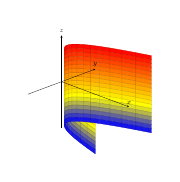
\begin{tikzpicture}[scale=0.25]
  \begin{axis}[
    view={45}{30},
    xlabel=$x$,
    ylabel=$y$,
    zlabel=$z$,
    axis lines=middle,
    ticks=none,
    enlargelimits=true,
    axis on top,
    z post scale=1.5,
    xlabel style={anchor=south},
    ylabel style={anchor=south},
    zlabel style={anchor=south},
    clip=false
]
  \addplot3[surf, domain=-1:1, y domain=-2:2, samples=20] ({cosh(x)}, {sinh(x)}, {y});
  \end{axis}
  \end{tikzpicture} \\
  \hline
  
  \textbf{Sinusoidal Surface} & \( z = \sin(x) + \cos(y) \) & Wavy grid & Periodic & 
  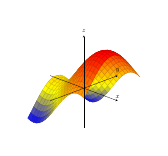
\begin{tikzpicture}[scale=0.25]
  \begin{axis}[
    view={45}{30},
    xlabel=$x$,
    ylabel=$y$,
    zlabel=$z$,
    axis lines=middle,
    ticks=none,
    enlargelimits=true,
    axis on top,
    z post scale=1.5,
    xlabel style={anchor=south},
    ylabel style={anchor=south},
    zlabel style={anchor=south},
    clip=false
]
  \addplot3[surf, domain=-2:2, samples=20] {sin(deg(x)) + cos(deg(y))};
  \end{axis}
  \end{tikzpicture} \\
  \hline
  \end{tabular}
  \caption{Common 3D surfaces with plots and key properties.}
  \end{table}
